\documentclass[unicode,mathserif]{beamer}

\usepackage[utf8]{inputenc}
\usepackage{cmap}
\usepackage[russian]{babel}

\usepackage{eulervm}
\usepackage{pifont}
\usepackage{mathtools}

\newcommand{\xmark}{\ding{56}}

% listings
\usepackage{listings}
\lstset{language=java,frame=shadowbox,rulesepcolor=\color{gray},
        resetmargins=true,showstringspaces=false,
        basicstyle=\ttfamily,keywordstyle=\color{blue},
        stringstyle=\color{purple},commentstyle=\color{gray},
        morekeywords={assert,enum,@interface}}

% beamer
\usetheme{CambridgeUS}

\beamertemplatenavigationsymbolsempty

\setbeamertemplate{bibliography item}[book]
\setbeamertemplate{bibliography entry note}{//~}
\setbeamercolor{bibliography entry note}{fg=structure}


\title[Многопоточность (1)]{Многопоточность в Java: основы}
\author{Алексей Владыкин}
\date{13 ноября 2017}

\begin{document}

\begin{frame}
\titlepage
\end{frame}

\begin{frame}
\tableofcontents
\end{frame}


\section{Общие сведения о параллелизме}

\begin{frame}
\centering

\includegraphics[width=0.8\textwidth]{pics/parallel.jpg}
\end{frame}


\begin{frame}{Мотивация}
\begin{itemize}
\item Одновременное выполнение нескольких действий\\
    (например, отрисовка пользовательского интерфейса
    и передача файлов по сети)
    \bigskip

\item Ускорение вычислений\\
    (при наличии нескольких вычислительных ядер)
\end{itemize}
\end{frame}


\begin{frame}{Закон Амдала}
$$S(N)=\frac{1}{(1-P)+\frac{P}{N}}$$
\bigskip
\begin{itemize}
\item $S$ --- ускорение (speedup)
\item $P$ --- доля вычислений, которые возможно распараллелить
\item $N$ --- количество вычислительных ядер
\end{itemize}
\end{frame}


\begin{frame}{Параллелизм в Java}
\begin{itemize}
\item Запуск нескольких JVM на одном или на разных компьютерах
    \begin{itemize}
    \item Нет общей памяти
    \item Взаимодействие через файловую систему или сетевое соединение
    \end{itemize}
    \bigskip
    \pause

\item Запуск нескольких потоков внутри JVM
    \begin{itemize}
    \item Есть общая память
    \item Обширная поддержка в языке и стандартной библиотеке
    \end{itemize}
\end{itemize}
\end{frame}


\section{Управление потоками}

\begin{frame}
\centering
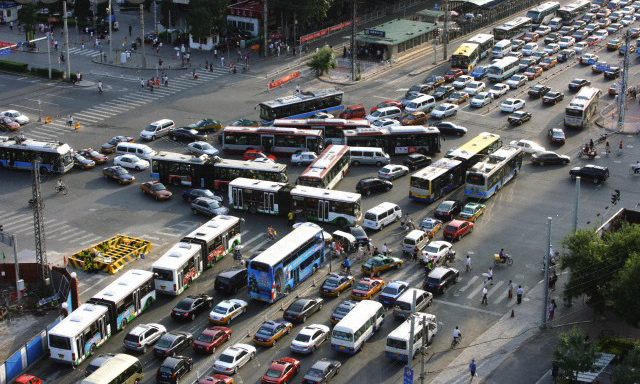
\includegraphics[width=0.9\textwidth]{pics/multithreading.jpg}
\end{frame}


\begin{frame}{\texttt{java.lang.Thread}}
\begin{itemize}
\item Потоки представлены экземплярами класса \texttt{java.lang.Thread}
    \bigskip

\item \lstinline|String getName()|
\item \lstinline|long getId()|
\item \lstinline|boolean isDaemon()|
\item \lstinline|StackTraceElement[] getStackTrace()|
\end{itemize}
\end{frame}


\begin{frame}{Thread dump}
\begin{itemize}
\item Список всех потоков с их состояниями и stack trace'ами
    \bigskip

\item \texttt{Ctrl+Break} или \texttt{Ctrl+\textbackslash}
\item \texttt{jps -l}, затем \texttt{jstack PID}
\item Кнопка в IDE
\end{itemize}
\end{frame}


\begin{frame}[fragile]{Создание потока: подкласс \texttt{Thread}}
\begin{lstlisting}
Thread thread = new Thread() {

    @Override
    public void run() {
        // do some work
    }
}
\end{lstlisting}
\end{frame}


\begin{frame}[fragile]{Создание потока: \texttt{Runnable}}
\begin{lstlisting}
Runnable runnable = () -> {
    // do some work
};

Thread thread = new Thread(runnable);
\end{lstlisting}
\end{frame}



\begin{frame}{Жизненный цикл потока}
\begin{itemize}
\item Создание объекта \texttt{Thread}
    \bigskip

\item Запуск\\
    \lstinline|thread.start()|
    \bigskip

\item Работа\\
    выполняется метод \lstinline|run()|,
    \lstinline|thread.isAlive() == true|
    \bigskip

\item Завершение\\
    метод \lstinline|run()| закончился или бросил исключение
    \bigskip

\item Завершенный поток нельзя перезапустить
\end{itemize}
\end{frame}


\begin{frame}{Прерывание потока}
\begin{itemize}
\item \lstinline|thread.interrupt()|
    \bigskip

\item Если поток находится в ожидании (\texttt{sleep}, \texttt{join}, \texttt{wait}),
    то ожидание прерывается исключением \texttt{InterruptedException}
    \bigskip

\item Иначе у потока просто устанавливается флаг \texttt{interrupted}
    \begin{itemize}
    \item флаг проверяется методами \lstinline|interrupted()|
            и \lstinline|isInterrupted()|
    \item проверять флаг и завершать поток надо самостоятельно
    \end{itemize}
    \bigskip

\item \lstinline|thread.join()|
\end{itemize}
\end{frame}



\section{Синхронизация потоков}

\begin{frame}
\centering

\includegraphics[width=0.5\textwidth]{pics/hope.jpg}
\end{frame}


\begin{frame}{Возможности встроенной синхронизации}
\begin{itemize}
\item Взаимное исключение\\
    (пока один поток что-то делает, другие не могут ему помешать)
    \bigskip

\item Ожидание и уведомление\\
    (поток ожидает уведомлений от других потоков)
\end{itemize}
\end{frame}


\begin{frame}[fragile]{Ключевое слово \texttt{synchronized}}
\begin{itemize}
\item Синхронизованный метод
    \begin{lstlisting}
    public synchronized void doSomething() {
        // ...
    }
    \end{lstlisting}
    \bigskip

\item Синхронизованный блок внутри метода
    \begin{lstlisting}
    public void doSomething() {
        synchronized (obj) {
            // ...
        }
    }
    \end{lstlisting}
\end{itemize}
\end{frame}


\begin{frame}{Ключевое слово \texttt{synchronized}}
\begin{itemize}
\item Синхронизация блоков --- по указанному объекту
    \bigskip

\item Синхронизация методов --- по текущему объекту (\lstinline|this|)
    \bigskip

\item Синхронизация статических методов --- по классу
\end{itemize}
\end{frame}


\begin{frame}{Взаимное исключение}
\begin{itemize}
\item Только один поток может исполнять метод или блок,
    синхронизированный по данному объекту
    \bigskip

\item Остальные потоки будут ждать
    \bigskip

\item Можно синхронизироваться на одном объекте,
    а по факту работать с другим
\end{itemize}
\end{frame}


\begin{frame}[fragile]{Взаимное исключение}
\begin{lstlisting}
class C {
    synchronized void foo() {}
    synchronized void bar() {}
    static synchronized void baz() {}
}
\end{lstlisting}
\begin{center}
\begin{tabular}{l|cccc}
    &\lstinline|c1.foo()| &\lstinline|c1.bar()| &\lstinline|c2.foo()| &\lstinline|C.baz()| \\
\hline
\lstinline|c1.foo()|&\xmark &\xmark \\
\lstinline|c1.bar()|&\xmark &\xmark \\
\lstinline|c2.foo()|&       &       &\xmark \\
\lstinline|C.baz()| &       &       &       &\xmark
\end{tabular}
\end{center}
\end{frame}


\begin{frame}{Ожидание и уведомления}
\begin{itemize}
\item Допустимо только внутри \lstinline{synchronized} по этому же объекту
    \bigskip

\item \lstinline|void wait()|\\
    \lstinline|void wait(long millis)|\\
    \lstinline|void wait(long millis, int nanos)|
    \bigskip

\item \lstinline|void notify()|\\
    \lstinline|void notifyAll()|
\end{itemize}
\end{frame}



\section{Модель памяти}

\begin{frame}
\centering

\includegraphics[width=0.5\textwidth]{pics/hardcore.jpg}

$$
\forall x, y \in A_i, z \in (C_i - C_{i-1}):
x\xrightarrow{ssw_i} y \xrightarrow{hb_i} z
\Rightarrow (\forall j \ge i: x \xrightarrow{sw_j} y)
$$
\end{frame}


\begin{frame}{Атомарность}
\begin{itemize}
\item Чтение и запись полей всех типов, кроме \lstinline|long|
    и \lstinline|double|, происходит атомарно
    \bigskip

\item Если поле объявлено с модификатором \lstinline|volatile|,
    то атомарно читаются и пишутся даже \lstinline|long|
    и \lstinline|double|
\end{itemize}
\end{frame}


\begin{frame}{Видимость}
\begin{itemize}
\item Изменения значений полей, сделанные одним потоком, могут быть не видны
    в другом потоке
    \bigskip

\item Изменения, сделанные одним потоком, могут быть видны в другом
    потоке в ином порядке
    \bigskip

\item Правила формализованы при помощи отношения \texttt{happens-before}
    \bigskip

\item Семантика \texttt{final}
\end{itemize}
\end{frame}


\begin{frame}{\texttt{happens-before}}
\begin{itemize}
\item Запись \lstinline|volatile|-поля \texttt{happens-before} чтения этого поля
    \bigskip

\item Освобождение объекта \texttt{happens-before} захват того же объекта
    \bigskip

\item \lstinline|thread.start()| \texttt{happens-before} \lstinline|thread.run()|
    \bigskip

\item Завершение \lstinline|thread.run()| \texttt{happens-before} 
    выход из \lstinline|thread.join()|
    \bigskip

\item \ldots
\end{itemize}
\end{frame}


\section{Советы}

\begin{frame}
\begin{itemize}
\item Четко разделяйте, где приватные данные потока,
    а где общие для нескольких потоков
\item Минимизируйте изменения состояния;\\
    подумайте о том, чтобы сделать свои объекты immutable
\item Инкапсулируйте синхронизацию в реализации класса
\item Если это невозможно, то явно документируйте требования к внешней
    синхронизации
\item Сначала сделайте программу правильной (и простой), а потом
    ускоряйте и распараллеливайте
\end{itemize}
\end{frame}

\end{document}

